\documentclass[]{article}
\usepackage[english, greek]{babel}
\usepackage[margin=2.5cm]{geometry}
\usepackage{fontspec}
\usepackage{graphicx}
\usepackage{subcaption}
\usepackage{listings}
\usepackage{float}
\usepackage{todonotes}
\usepackage{hyperref}

% Define custom colors
\definecolor{codegreen}{rgb}{0,0.6,0}
\definecolor{codegray}{rgb}{0.5,0.5,0.5}
\definecolor{codepurple}{rgb}{0.58,0,0.82}
\definecolor{backcolour}{rgb}{0.95,0.95,0.92}

% Setup the language and colors
\lstset{
	language=Python,
	backgroundcolor=\color{backcolour},   
	commentstyle=\color{codegreen},
	keywordstyle=\color{magenta},
	numberstyle=\tiny\color{codegray},
	stringstyle=\color{codepurple},
	basicstyle=\ttfamily\footnotesize,
	breakatwhitespace=false,         
	breaklines=true,                 
	keepspaces=true,                 
	numbers=left,                    
	numbersep=5pt,                  
	showspaces=false,                
	showstringspaces=false,
	showtabs=false,                  
	tabsize=2,
}

%opening
\title{\textbf{Όραση Υπολογιστών}\\ 2η Σειρά Εργαστηριακών Ασκήσεων}
\author{Ραφτόπουλος Μιχαήλ - ΑΜ: 03120114}
\date{Εαρινό Εξάμηνο 2024}

\begin{document}
	\setmainfont{Liberation Serif}
	\maketitle
	
	\section*{Μέρος 1: Παρακολούθηση Προσώπου και Χεριών με Χρήση της Μεθόδου Οπτικής Ροής των Lucas-Kanade}
	\subsection*{1.1 Ανίχνευση Δέρματος Προσώπου και Χεριών}
	\paragraph{1.1.1} Υλοποιήθηκε η συνάρτηση SkinDetect(), που εντοπίζει τις περιοχές δέρματος και επιστρέφει μια λίστα αό τα αντίστοιχα bounding boxes. Να σημειωθεί ότι χρειάστηκε αρκετά μικρότερο threshold από το προτεινόμενο, με τιμή $threshold = 0.0005$.
	\begin{figure}[h]
		\centering
		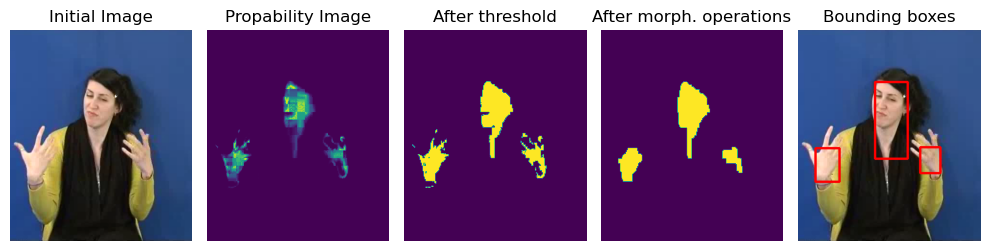
\includegraphics[width=\linewidth]{1_1}
		\caption{Στάδια εντοπισμού περιοχών δέρματος}
	\end{figure}
	\subsection*{1.2 Παρακολούθηση Προσώπου και Χεριών}
	\paragraph{1.2.1} Έγινε η υλοποίηση του μονοκλιμακωτού Lucas Kanade. Πριν τρέξουμε τον αλγόριθμο, διευρύνουμε το bounding box κατά 20 pixels, ώστε να είναι πιο "ανθεκτικός" σε απότομες κινήσεις. Παρατηρώντας του αποτέλεσμα, βλέπουμε ότι τα μεγαλύτερα διανύσματα οπτικής ροής έχουν σχετικά σωστή κατεύθυνση, συνολικά όμως τα διανύσματα είναι αρκετά ανοργάνωτα.
	\begin{figure}[h]
		\centering
		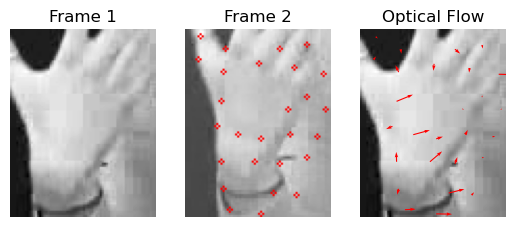
\includegraphics[width=0.5\linewidth]{1_2_1}
		\caption{Frame 1, frame 2 με σημειωμένες τις γωνίες, frame 1 με σημειωμένα τα διανύσματα οπτικής ροής}
	\end{figure}
	\paragraph{Παρατηρήσεις: }
	\begin{itemize}
		\item Μειώνοντας την παράμετρο $\epsilon$, το αποτέλεσμα γίνεται υπερβολικά ασταθές. Διατηρείται λοιπόν στην μεγαλύτερη προτεινόμενη τιμή, $\epsilon = 0.1$.
		\item Η μεταβολή στο $\rho$ επηρεάζει λιγότερο το τελικό αποτέλεσμα. Αυξάνοντάς το φαίνεται να αυξάνονται τα outliers, αλλά με μικρή διαφορά.
	\end{itemize}
	\paragraph{1.2.2} Υλοποιήθηκε η συνάρτηση υπολογισμού της ολικής οπτικής ροής. Χρησιμοποιήθηκαν δύο μέθδοι: απλή μέση τιμή και μέση τιμή μετά από εφαρμογή άνω κατωφλίου. Το κατώφλι έχει τιμή τριπλάσια από τη μέση ενέργεια των διανυσμάτων οπτικής ροής. Ύστερα, για κάθε εικόνα εισόδου, βρέθηκε η οπτική ροή και σχεδιάστηκε μαζί με το κατάλληλα μετατοπισμένο bounding box. Οι εικόνες εξόδου μπορούν να βτεθούν στον φάκελο 'part1\_output/1\_2\_2. Το tracking είναι επιτυχημένο μέχρι και το frame 27, όπου η διερμηνέας κάνει μια απότομη κίνηση με τα χέρια. Από εκείνο το σημείο και μετά, το tracking στα χέρια αποτυγχάνει.
	\paragraph{1.2.3} Υλοποιήθηκε η πολυκλιμακωτή εκδοχή του Lucas Kanade, σε 5 κλίμακες. Δοκιμάζοντάς την πρώτα σε δύο frames, βλέπουμε επιτόπου μεγάλη βελτίωση. Τα διανύσματα οπτικής ροής δείχνουν προς τη σωστή κατεύθυνση, είναι παράλληλα μεταξύ τους και έχουν ίδιο μήκος.
	\begin{figure}[h]
		\centering
		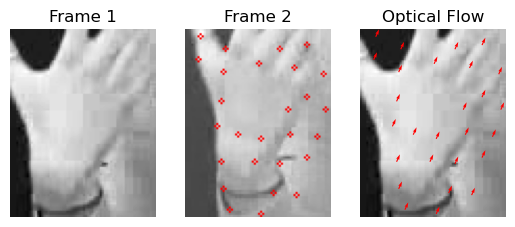
\includegraphics[width=0.5\linewidth]{1_2_3}
		\caption{Frame 1, frame 2 με σημειωμένες τις γωνίες, frame 1 με σημειωμένα τα διανύσματα οπτικής ροής}
	\end{figure}
	\paragraph{} Δοκιμάζουμε τον αλγόριθμο σε όλες τις εικόνες εισόδου. 
	
	\section*{Μέρος 2: Εντοπισμός Χωρο-χρονικών Σημείων Ενδιαφέροντος και Εξαγωγή Χαρακτηριστικών σε Βίντεο Ανθρωπίνων Δράσεων}
	\subsection*{2.1 Χωρο-χρονικά Σημεία Ενδιαφέροντος}
	\paragraph{2.1.1}
	\paragraph{2.1.2} 
	\paragraph{2.1.3} 
	\paragraph{2.1.4} 
	\subsection*{2.2 Χωρο-χρονικοί Ιστογραφικοί Περιγραφητές}
	\paragraph{2.2.1} 
	\paragraph{2.2.2}
	\subsection*{2.3 Κατασκευή Bag of Visual Words και χρήση Support Vector Machines για την ταξινόμηση δράσεων}
	\paragraph{2.3.1} 
	\paragraph{2.3.2} 
	\paragraph{2.3.3}
	\paragraph{2.3.4}
	
	\section*{Μέρος 3: Συνένωση Εικόνων (Image Stitching) για Δημιουργία Πανοράματος}
	\subsection*{Βήμα 0}
	\paragraph{}
	\subsection*{Βήμα 1}
	\paragraph{}
	\subsection*{Βήμα 2}
	\paragraph{}
	\subsection*{Βήμα 3}
	\paragraph{}
	\subsection*{Βήμα 4}
	\paragraph{}
	\subsection*{Βήμα 5}
	\paragraph{}
	\subsection*{Βήμα 6}
	\paragraph{}
\end{document}
